\documentclass[12pt]{article}
\usepackage[utf8]{inputenc}      % For UTF-8 support
\usepackage[T1]{fontenc}
\usepackage{lmodern}
\usepackage{geometry}
\usepackage{booktabs}            % For nicer tables
\usepackage{hyperref}            % For hyperlinks in the document
\usepackage{graphicx}            % For images
\usepackage{array}               % For extended table features
\usepackage{setspace}
% \usepackage{xcolor}
% \pagecolor{gray}      % Set background color to black
% \color{white}          % Change text color to white
\usepackage{helvet}
\renewcommand{\familydefault}{\sfdefault}
\geometry{margin=1in}
\setstretch{1.15}
% \title{This is Main title \\ [0.2em]\large This is Subtitle}
% \title{Used Car Characteristics \\ [0.2em]\large An Explanatory Data Analysis}
% \author{Dávid Fodor \and Faisal Zayeem Ahmed \and Márió Palágyi}
% \date{Submission date: TBD}

\begin{document}

\begin{titlepage}
  \centering
  \vspace*{1in}
  {\Huge\bfseries Used Car Characteristics\par}
  \vspace{0.5em}
  {\Large An Explanatory Data Analysis\par}
  \vspace{1.5in}
  {\Large Dávid Fodor \\ Faisal Zayeem Ahmed \\ Márió Palágyi\par}
  \vfill
  {\large Submission date: TBD\par}
  \vspace{0.5in}
  {\large Datascience Capstone Project - IMC Krems}  % Optional: use the current date
\end{titlepage}

\section*{Abstract}
A brief overview of the project, including problem statement, methodology, key findings, and conclusions.

\section{Introduction}
\textbf{Problem Statement:} Describe the problem.\\[1ex]
\textbf{Objectives:} List the objectives and tasks required to be completed.\\[1ex]
\textbf{Data:} Describe your dataset.\\[1ex]
\textbf{Background Information:} Provide context and challenges based on your understanding of the problem.

\section{Literature Review}
Summary of relevant research and related works in the field. This section does not need to be exhaustive; include background knowledge on how the problem has been addressed before and how you plan to solve it.

Luckily, there is plenty of literature on the topic of used car prices, particularly the prediction car prices seems to be a popular topic. Searching on Google Scholar for "used car price prediction" yields almost a million results.

\begin{figure}[ht]
  \centering
  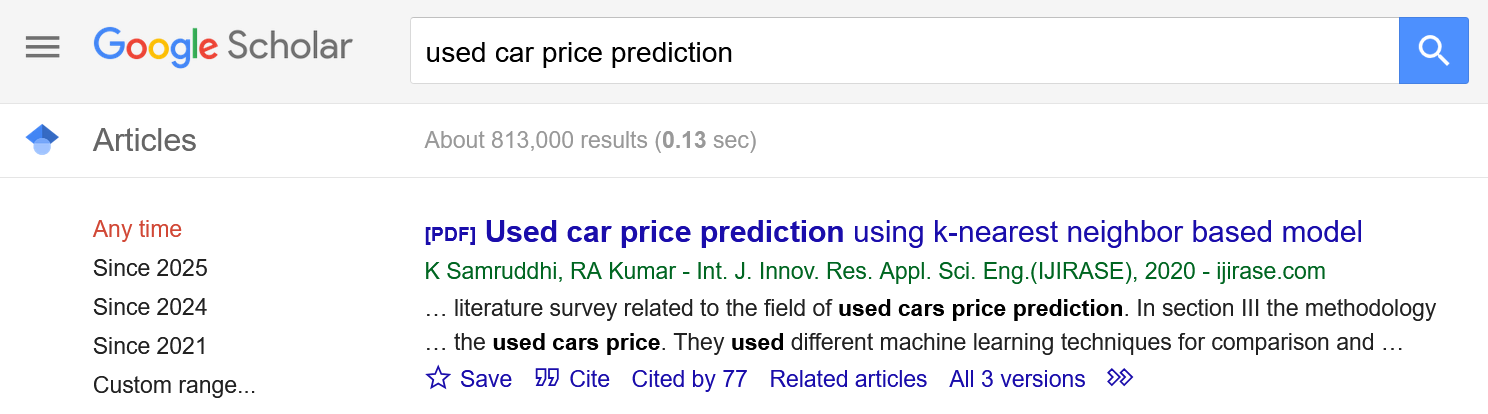
\includegraphics[width=0.8\textwidth]{./images/google_scholar.png}
  \caption{Screenshot of Google Scholar Search}
  \label{fig:google_scholar}
\end{figure}

\section{Methodology}
\begin{itemize}
    \item \textbf{Data Collection, Description and Management:} Describe the steps involved in data collection or preprocessing, including EDA.
    \item \textbf{Analysis Techniques:} Describe your approach to solving the problem. You can include a model diagram to illustrate your method.
    \item \textbf{Tools and Software Used:} List the tools, frameworks, and software used for the project.
\end{itemize}
\subsection{Data Collection}
In our case the data collection is a rather interesting part of the project, which took quite some time. Unlike other groups, we had to find our own primary datasource, seeking a used car marketplace which we could scrape.
After several trials of scraping different websites, we finally ended up with one that was quite lenient with their robots.txt file, and we could scrape it without any issues. The website we used was \url{https://www.autoscout24.com/}, which is one of the largest used car marketplaces in Europe boasting more than 2 million listings.

\begin{figure}[ht]
  \centering
  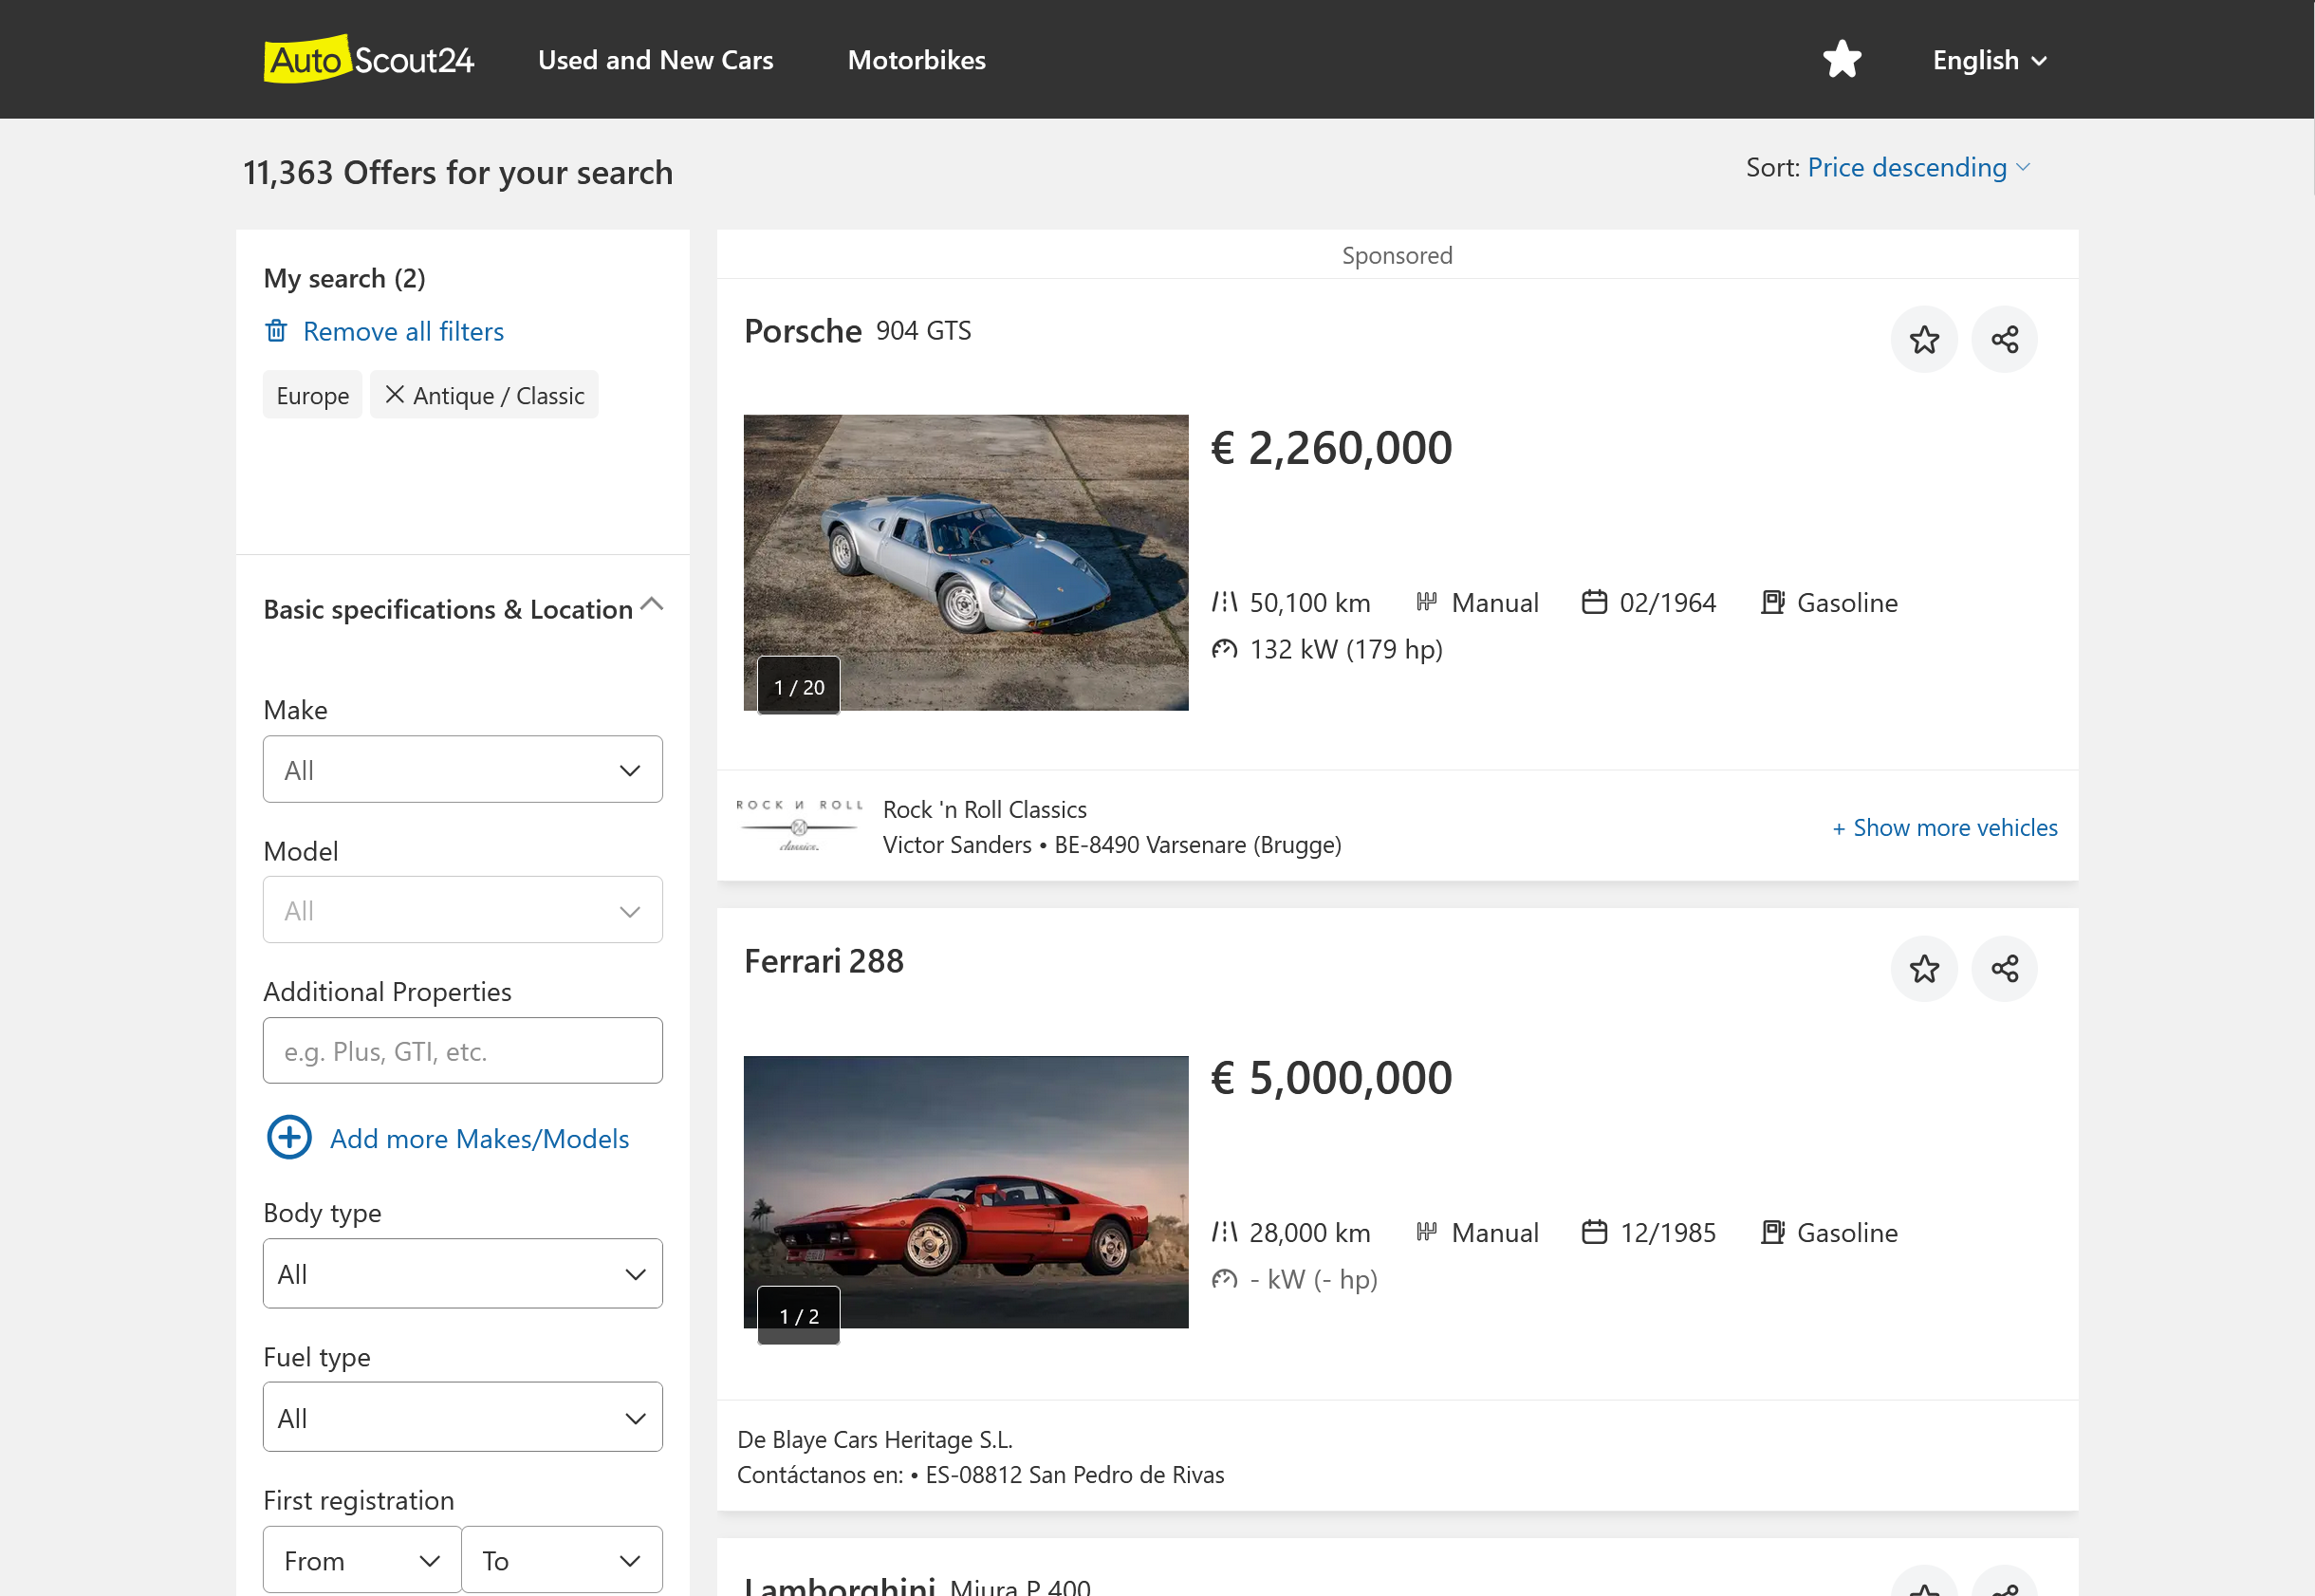
\includegraphics[width=0.8\textwidth]{./images/autoscout.png}
  \caption{Screenshot of Autoscout24 Homepage}
  \label{fig:autoscout}
\end{figure}

The scraping took place from \date{2025-04-03} to \date{2025-04-08}, running practically 24/7 on a laptop even though parallelization was used. In the end we have collected \textbf{505804} rows of data, which is a lot more than we could have hoped for in, and wrote it to a \textbf{parquet} file. The scraping consisted of two main parts, which we will discuss in the following subsections along with the bigger challanges we have faced.

\begin{figure}[ht]
  \centering
  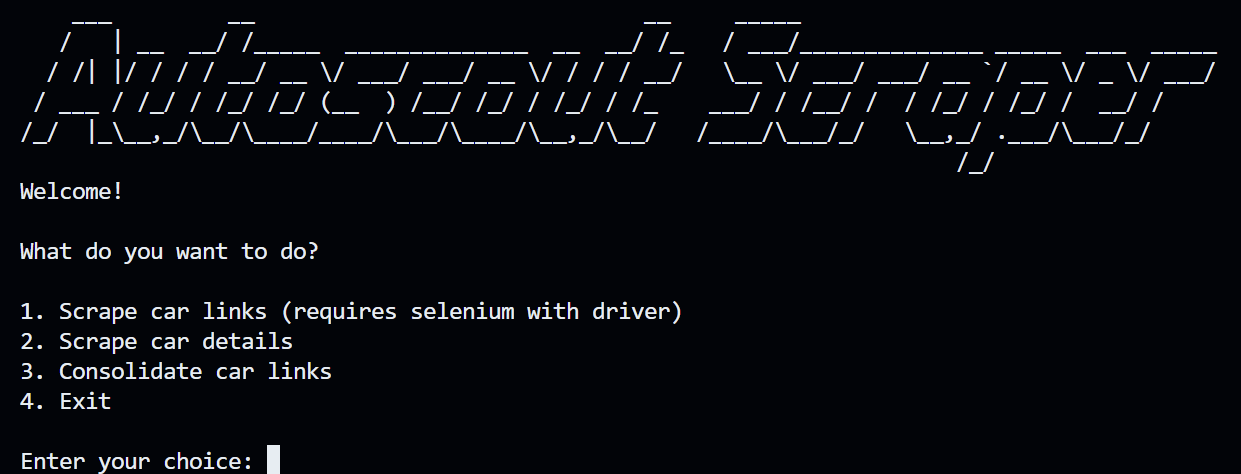
\includegraphics[width=0.8\textwidth]{./images/autoscout_scraper.png}
  \caption{Screenshot of Autoscout Scraper}
  \label{fig:autoscout_scraper}
\end{figure}

\subsubsection{Scraping Car Listing}

Due to the nature of the website, we needed user interaction for scraping the car listing, so we used \textbf{Selenium} to scrape the URLs pointing to specific car listings. This was achieved through a headless Chromium browser.
We faced two hurdles in this change which we had to overcome with simulated interactions.

\begin{itemize}
  \item \textbf{Pagination:} The website uses a classic pagination system on page, meaning we needed to be able to navigate through each page.
  \item \textbf{Max 20 pages per search:} The website limits the number of returned pages to 20, so we had to find a way to methodically filter search parameters to find as many sets of 20 pages as possible.
\end{itemize}

In theory almost every common feature of cars can be filtered on the page, so with enough patience one may find all 2 million listings. However, we did not have so much time, nor so many cores on our hands, so we tried finding a middle ground, which was the following:

\begin{enumerate}
  \item Loop through each car make available
  \item For each car make, loop through a range of dynamically changing power ranges in kw based on their presumed likelihood e.g. 0-15, 15-20, 20-25, 25-26, 26, 27\dots
  \item For each power range of the car make, loop through the pages available of the pagination
  \item On each pagination page, collect the URLs of the car listings
  \item Store the URLs in a JSON file, keyed by the make
\end{enumerate}

This constituted most of our time scraping, as the user interaction needed to be waited upon and there were simply a lot of possible permutations of make, power, pagination possibilities to go through.
We of course parallelized and worked on multiple cores, also introducing shortcuts, e.g. if we found a make with less than 500 lisitng we did not need to loop through power ranges at all.

\subsubsection{Scraping Car Details}

Once we have collected all the car URLs, the scraping was quite straightforward. We have tested the scraping on individual listings first, trying to find out what categories of data we can scrape and how we may achieve that. At this stage, we were lucky, as no user interaction was needed at all, not even for \textbf{declining cookies}, as the underlying HTML structure already contained the data we needed.
This allowed for us to scrape the data in a much more efficient way, as we could simply use the \textbf{requests} package and \textbf{BeautifulSoup} to parse the HTML and extract the data we needed. This had much lower overhead and allowed us to scrape more listings simultaneously. First fetching into a list in memory, then converting to a df, to then export into a \textbf{parquet} file.

Interesting to note that between the two scraping phases, many links seem to have moved, perhaps due to being sold, or delisted so this case also needed to be addressed.

\subsection{Preprocessing}

Preoprocessing was...

\section{Results}
Describe experiments and the evaluation protocol. Include tables, graphs, and charts as needed to present your findings and results.

\section{Discussion}
Interpret and analyze the results, and discuss possible future work and improvements.

\section{Conclusion}
Provide a summary of the project, key findings, and recommendations. (Approximately 200--350 words.)

\section{Bibliography}
Include relevant references such as websites, blogs, articles, research papers, etc.

\section{Self-Reflection}
Add a paragraph or half-page note reflecting on the project.

\end{document}